% Print results for comparing MSN with 2D Runge function

\begin{figure}[p]
    \centering
    \begin{subfigure}{0.45\textwidth}
    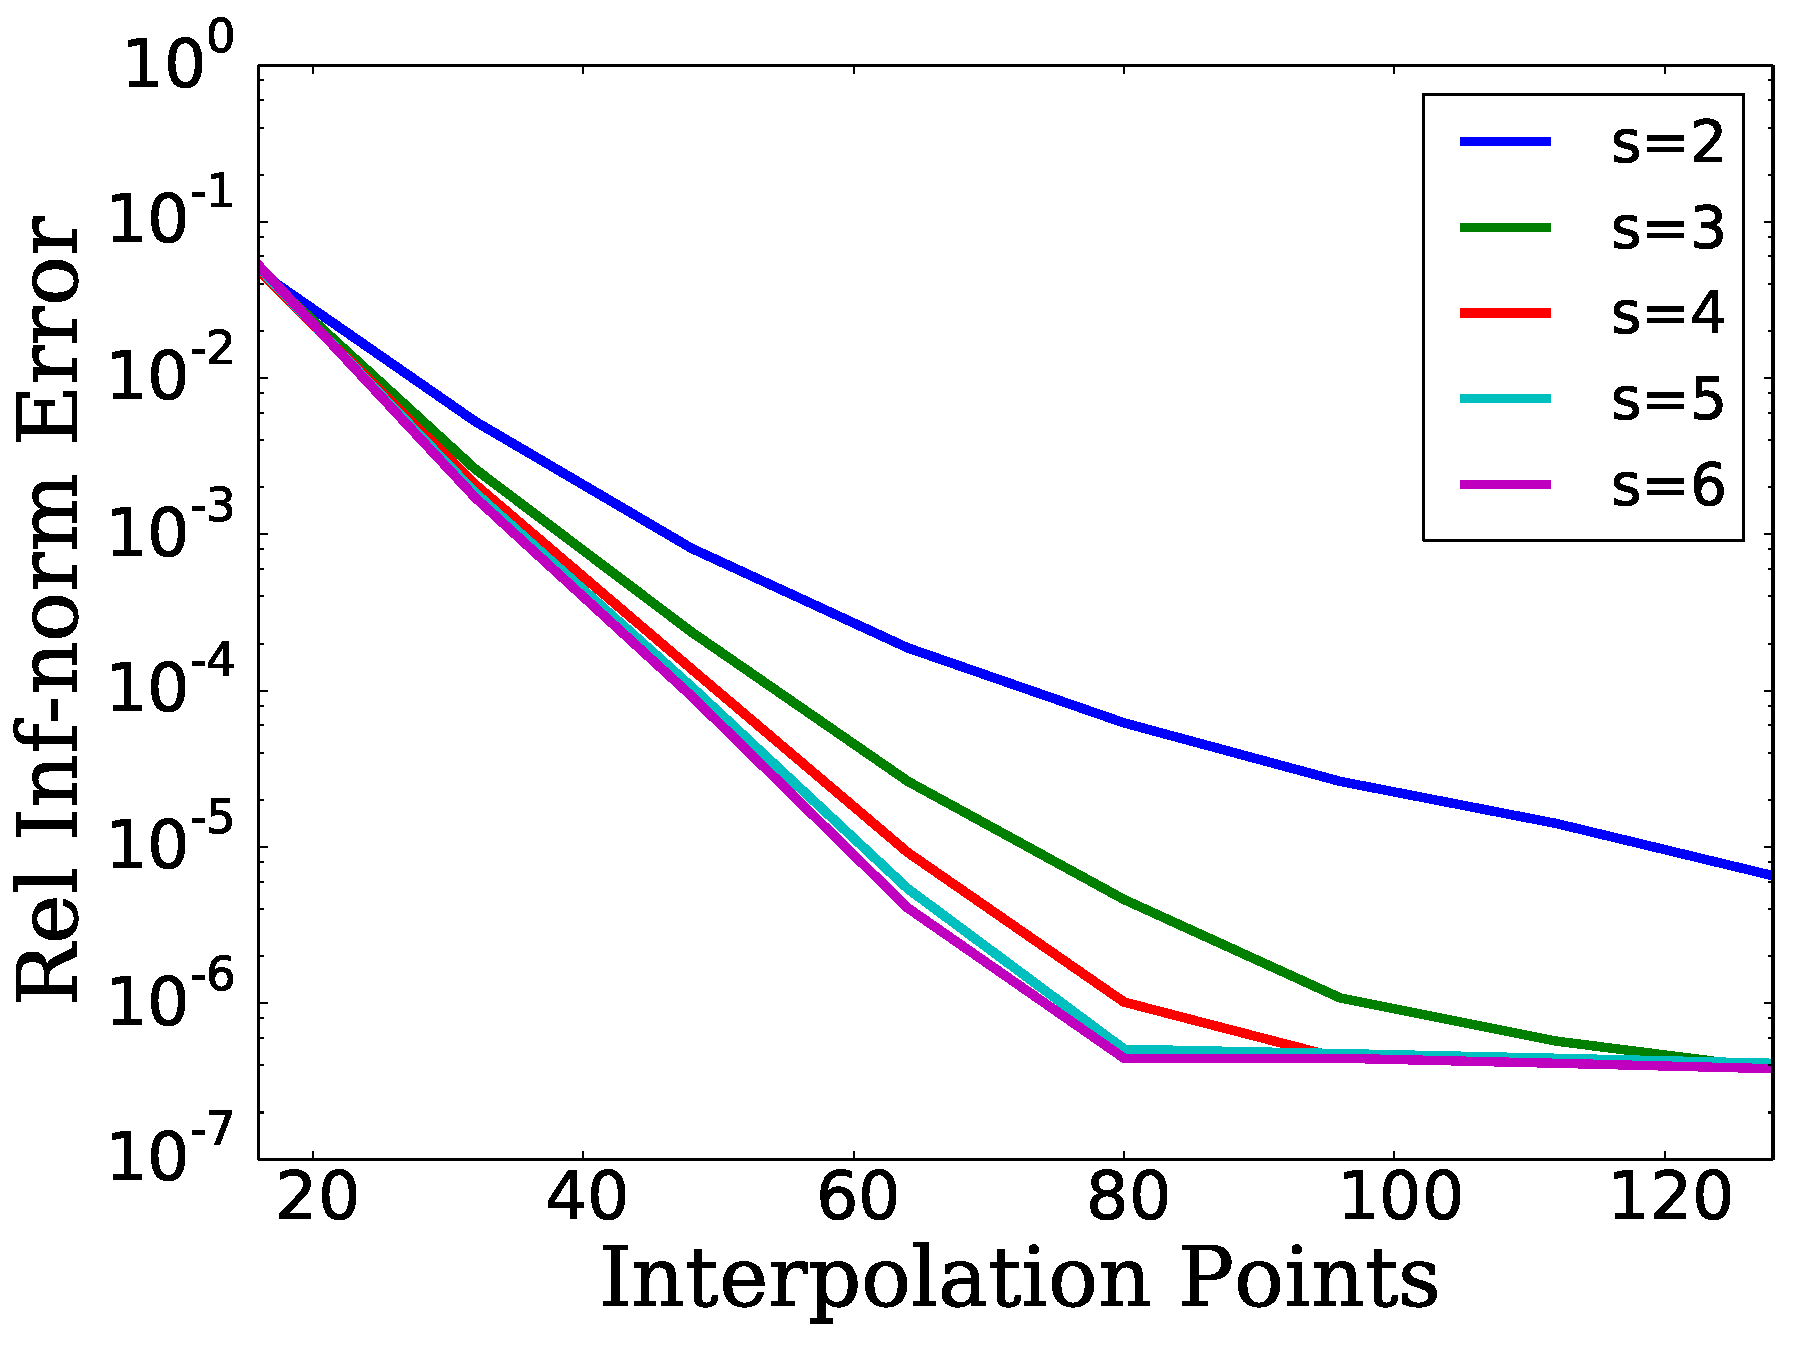
\includegraphics[width=\textwidth]{plots/msn_2n_fast_smooth_R_25_single.pdf}
    \caption{Single Precision}
    \end{subfigure}
    \begin{subfigure}{0.45\textwidth}
    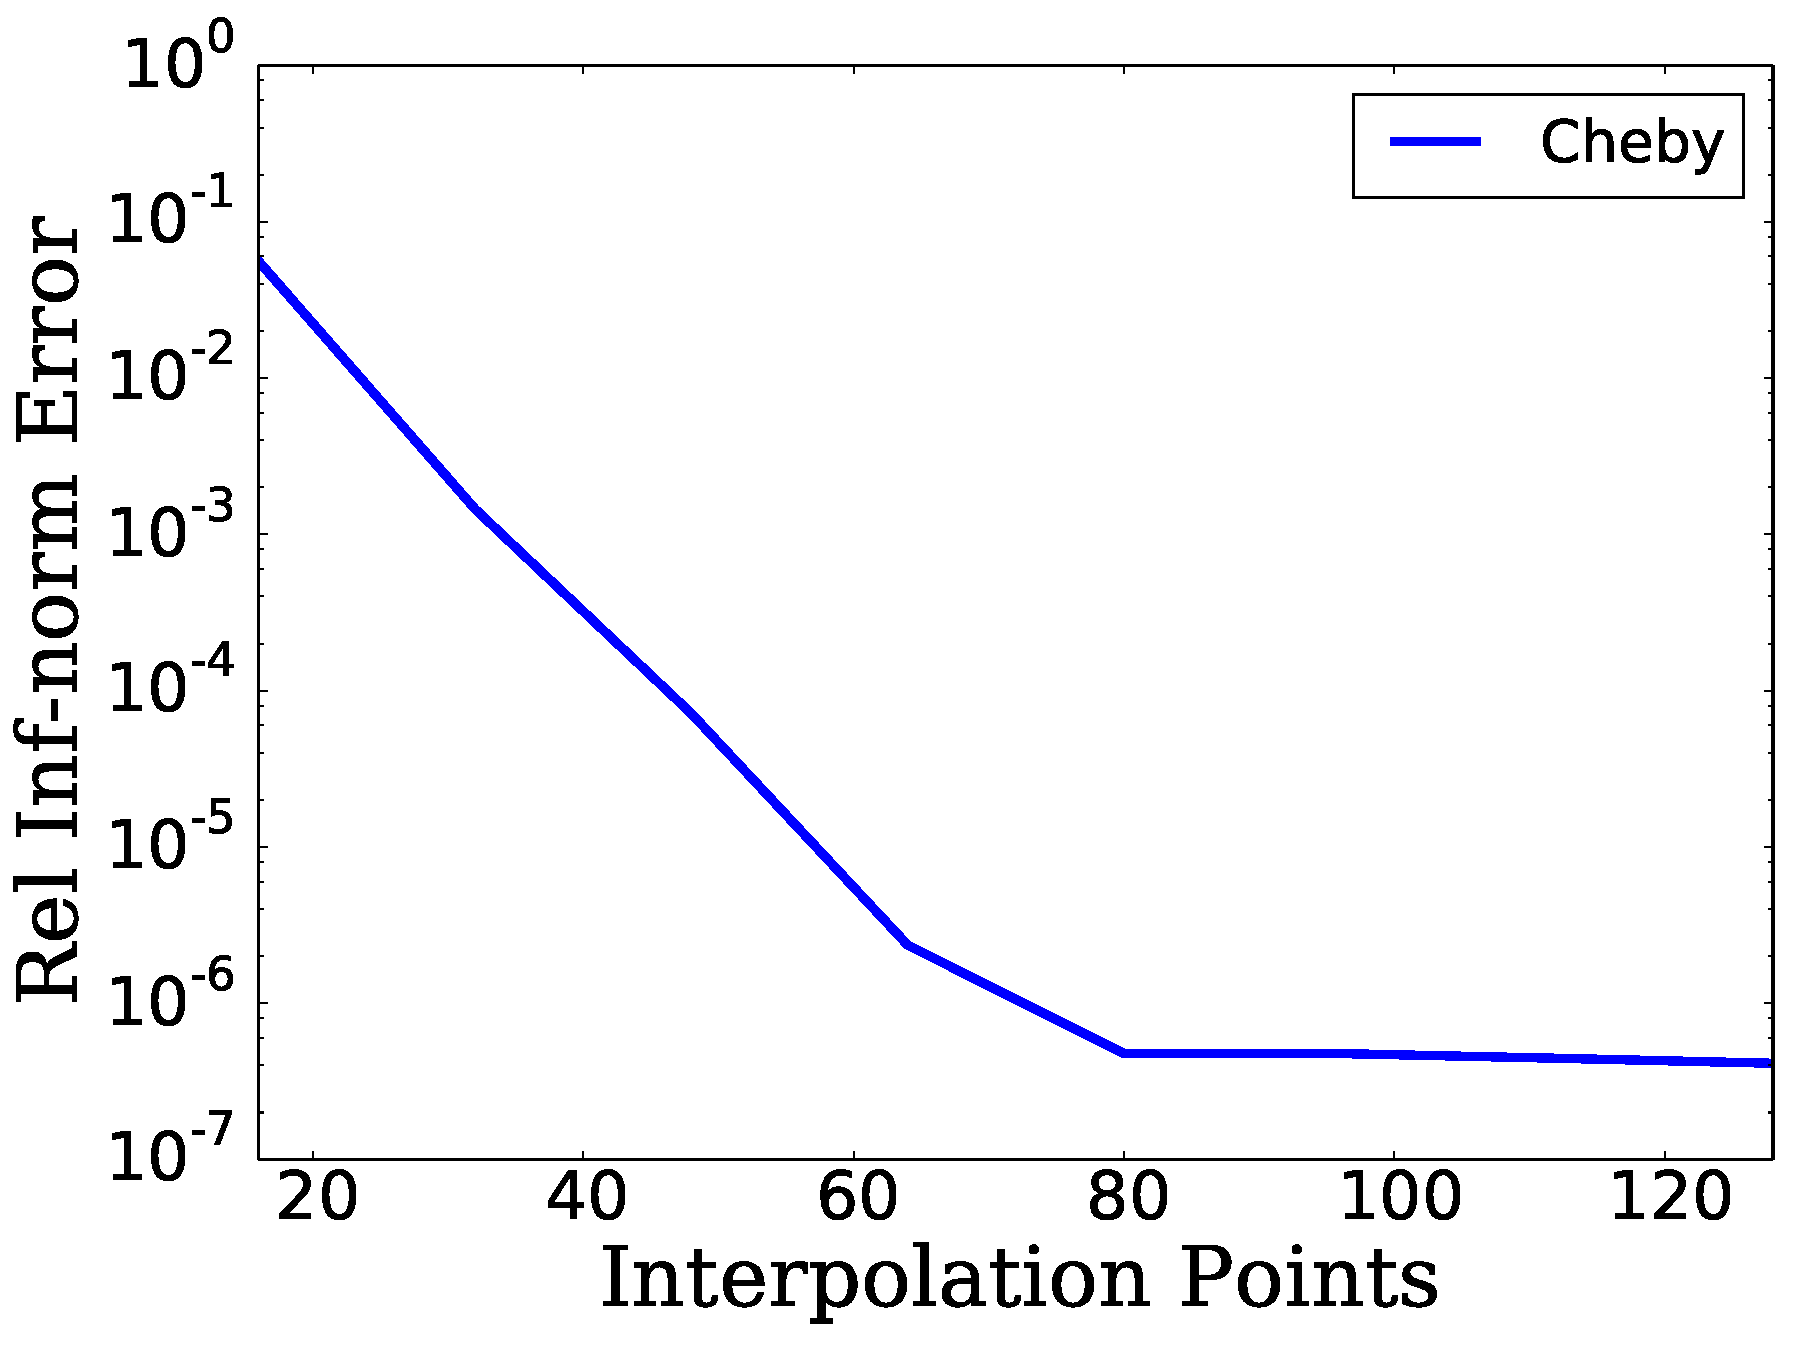
\includegraphics[width=\textwidth]{plots/cheby_interp_smooth_R_25_single.pdf}
    \caption{Single Precision}
    \end{subfigure}

    \begin{subfigure}{0.45\textwidth}
    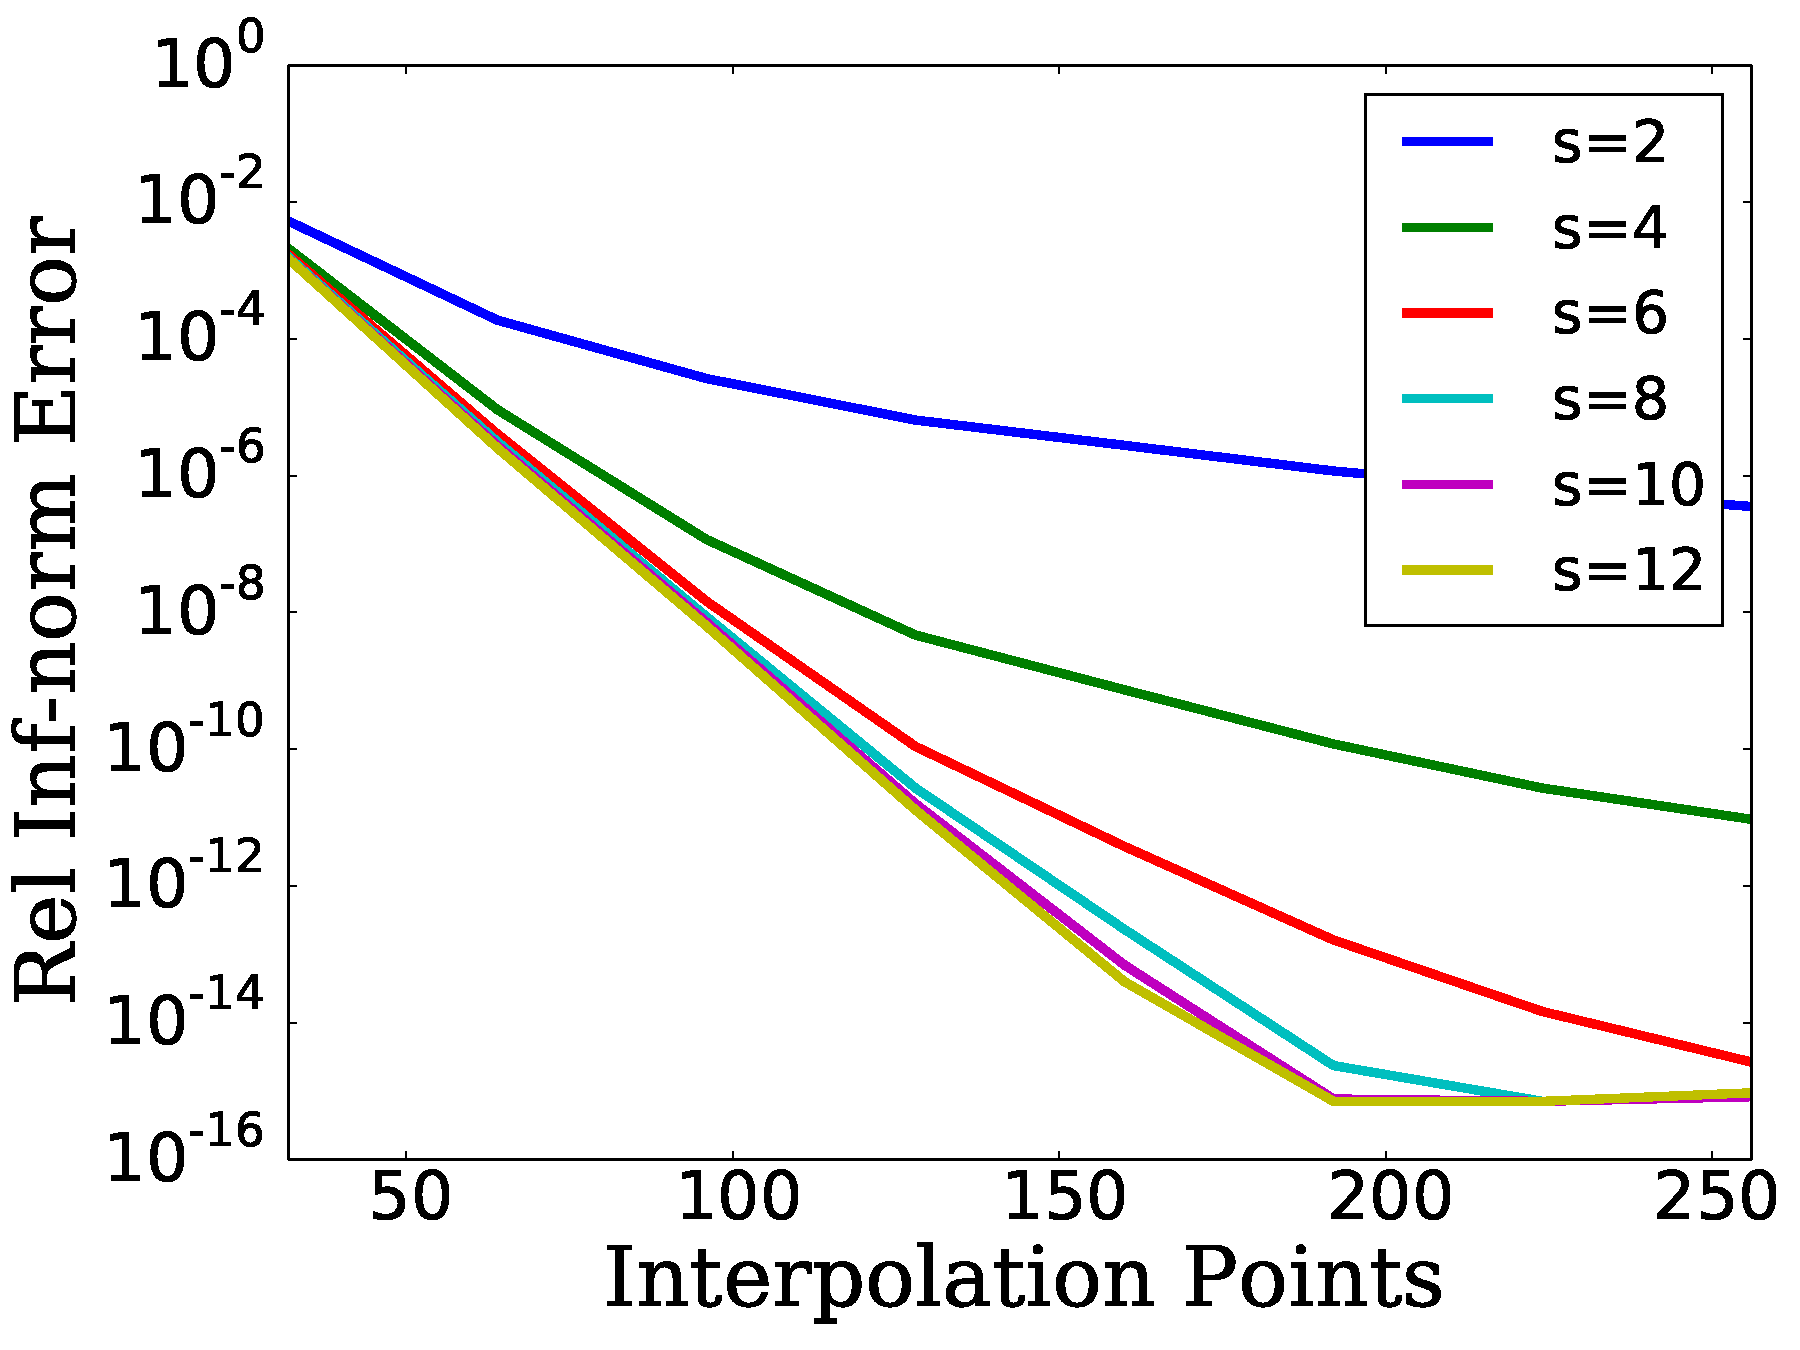
\includegraphics[width=\textwidth]{plots/msn_2n_fast_smooth_R_25_double.pdf}
    \caption{Double Precision}
    \end{subfigure}
    \begin{subfigure}{0.45\textwidth}
    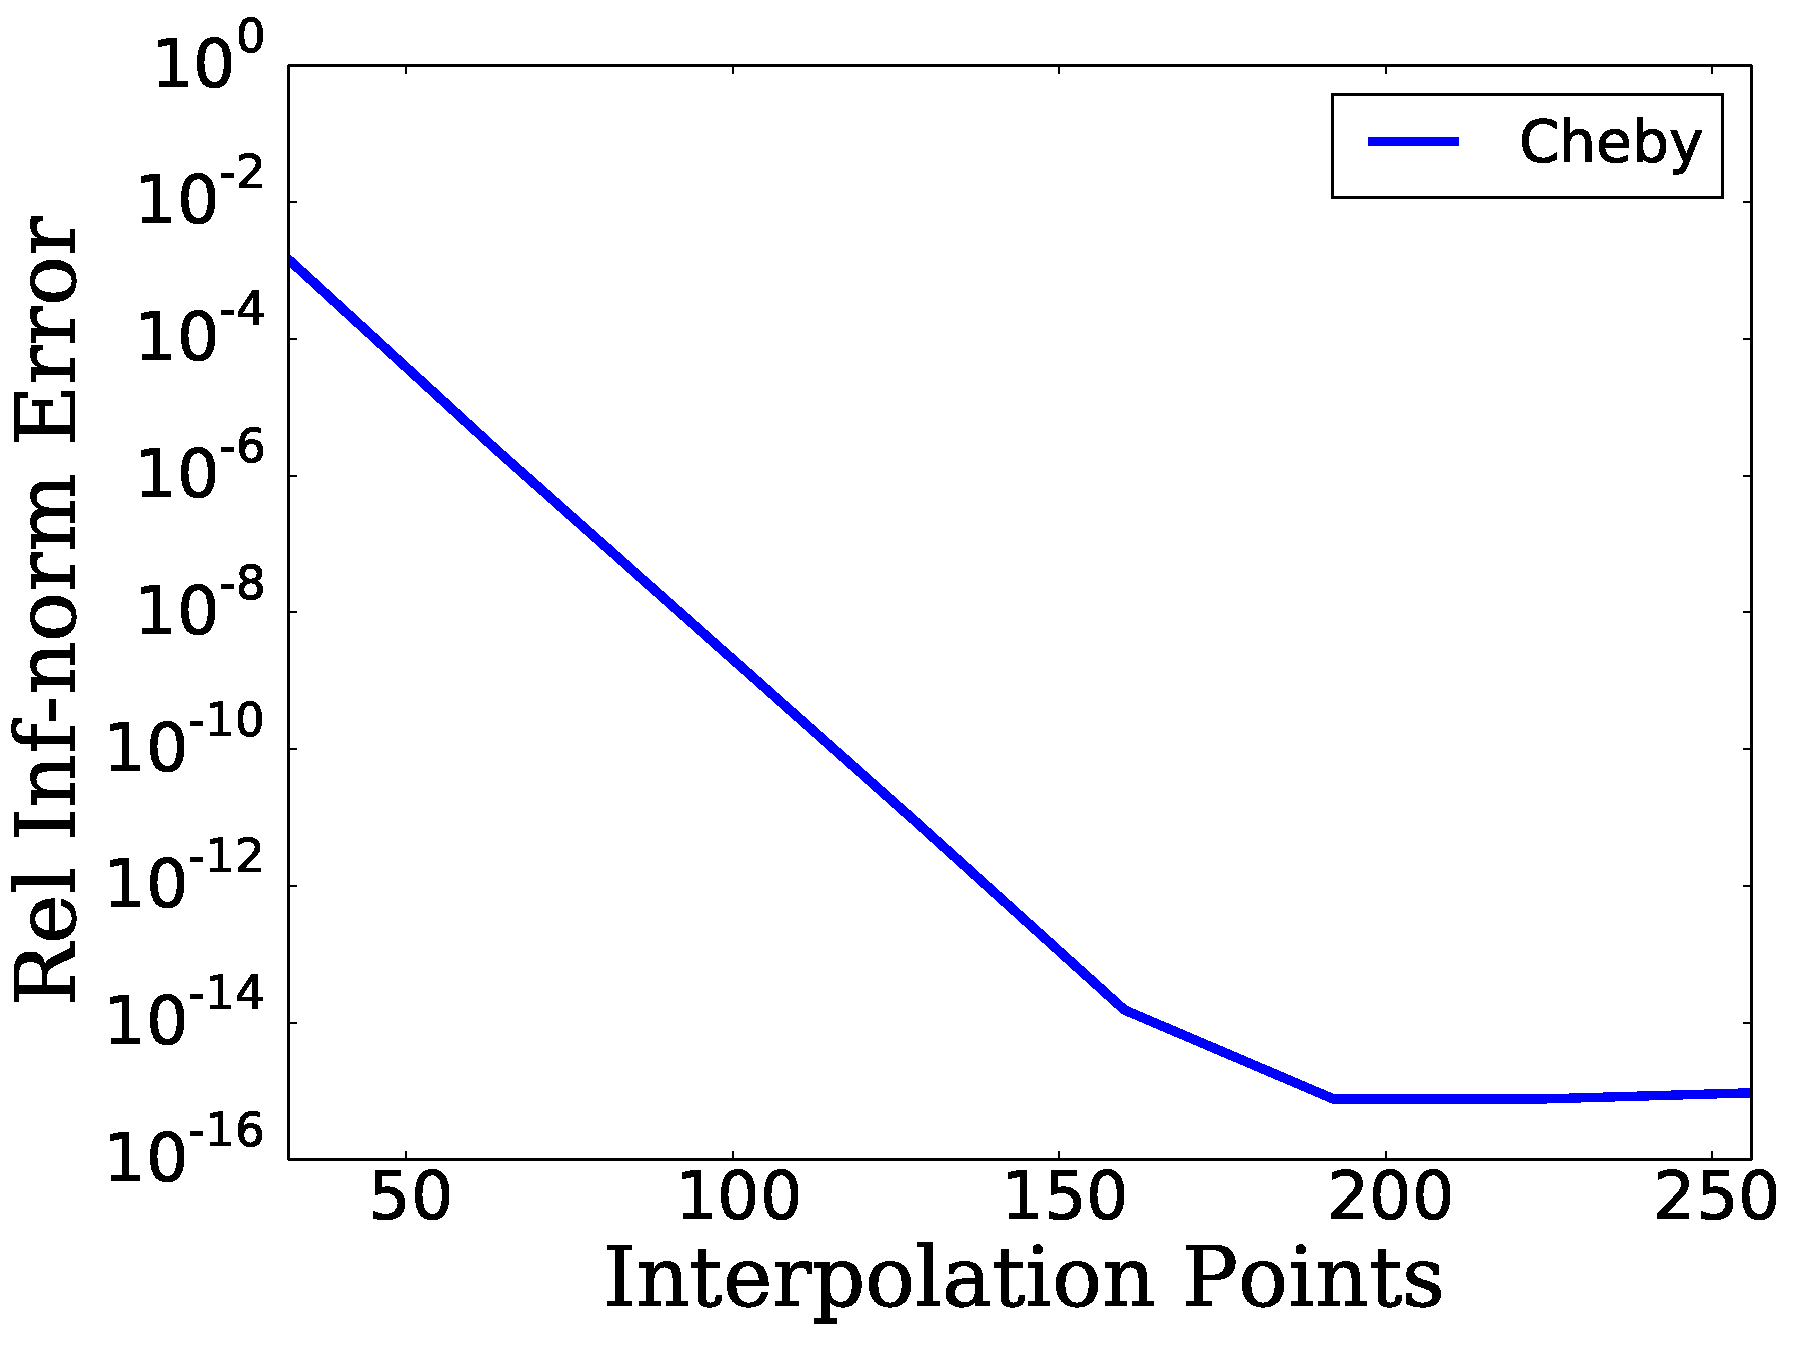
\includegraphics[width=\textwidth]{plots/cheby_interp_smooth_R_25_double.pdf}
    \caption{Double Precision}
    \end{subfigure}
\caption[Smooth Interpolation Comparison: 2D Runge Function $R=25$]{
MSN interpolation and Chebyshev interpolation results
of the 2D Runge function $f_{25}$ for various $s$ values.
Here, $n$ interpolation points refers to interpolation on the $n\times n$
tensor grid of Chebyshev points.
}
\label{fig:smooth_comparison_2d_runge_25}
\end{figure}



